% Follow-up experiments: numerical sensitivity and optimizer budget.
\begin{frame}{Could the Optimization Method Limit the Fit?}
\small
\begin{enumerate}
\item Perturb each of the four search coordinates in both directions, at three sizes and three solver timesteps.
\item Repeat both objectives with four starts and a larger evaluation budget, keeping the model, bounds and measured inputs fixed.
\item Try finite-difference L-BFGS-B near each previous candidate, then replay its best sampled point at smaller timesteps.
\end{enumerate}
\[
\frac{\partial f_i}{\partial u_j}\approx
\frac{f_i(u+h e_j)-f_i(u-h e_j)}{2h}
\]
\footnotesize
\(u\) contains normalized logarithms of \(C,S_e,C_{th}/S_e,\gamma\).
\(e_j\) changes one coordinate; \(h=0.001,0.005,0.02\) is a fraction of its log range.
\par\vspace{0.15cm}
A missing target frequency makes the full loss undefined. A finite penalty lets the search continue, but its slope is not the derivative of that loss.
\slidesource{Controlled optimizer follow-up, 20 October 2026. Same feature extraction and physical equations as the preceding comparison.}
\end{frame}


\begin{frame}{How Smoothly Does the Extracted Frequency Change?}
\centering
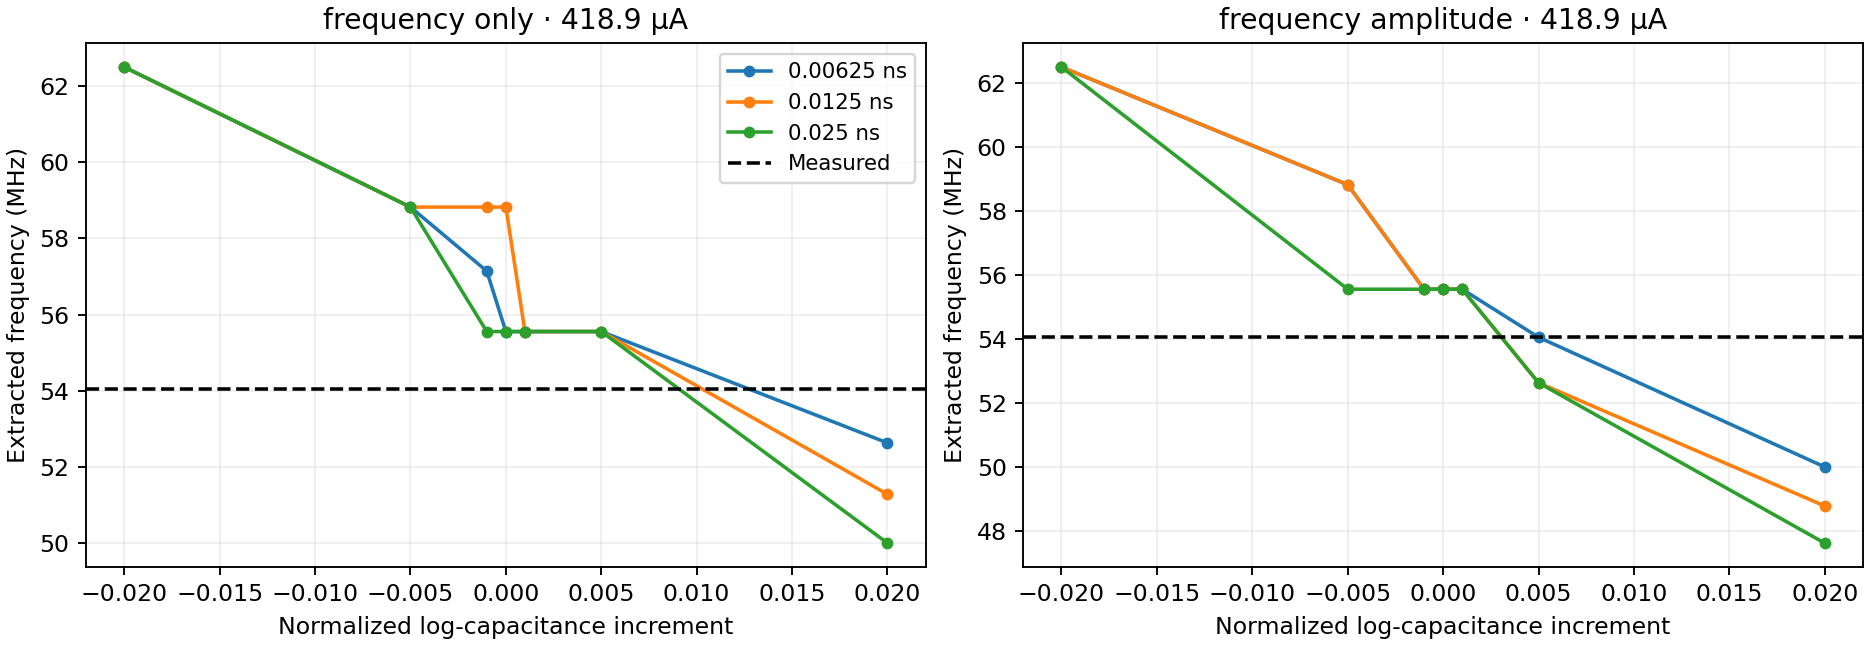
\includegraphics[width=0.96\linewidth]{../public_jobs/20261020_195947_optimizer-budget-derivative-and-gradient-review_555769/figures/frequency_profiles.png}
\par\footnotesize
Small parameter changes can leave the extracted frequency unchanged; larger changes move detected peak times. The curves also depend on the solver timestep.
\par\vspace{0.12cm}
644/792 individual-frequency difference estimates were defined; 327 were zero.
None of 72 full-loss difference estimates was defined, because at least one target frequency was missing.
\slidesource{Middle measured input: 418.9 \(\mu\)A. Acquisition grid: 1 ns; frequency from detected complete-cycle periods. Bundle 555769.}
\end{frame}

\begin{frame}{Larger Searches and Short Gradient Trials: Results}
\centering\footnotesize
\renewcommand{\arraystretch}{1.15}
\begin{tabular}{@{}llrrr@{}}
\toprule
\textbf{Objective} & \textbf{Method} & \textbf{Passing} & \textbf{Frequency error} & \textbf{Vpp error}\\
\midrule
Frequency only & Previous & 10/11 & 14.5\% (10/11) & 1965.7\% \\
Frequency only & Larger search & 10/11 & 14.5\% (10/11) & 1965.7\% \\
Frequency only & Gradient sample & 10/11 & 12.0\% (10/11) & 1979.8\% \\
\midrule
Frequency + Vpp & Previous & 8/11 & 18.2\% (9/11) & 903.0\% \\
Frequency + Vpp & Larger search & 10/11 & 14.5\% (10/11) & 1965.7\% \\
Frequency + Vpp & Gradient sample & 9/11 & 14.2\% (9/11) & 1195.5\% \\
\bottomrule
\end{tabular}
\par\vspace{0.16cm}\scriptsize
Errors: MAPE at 0.00625 ns. Frequency uses defined records (count shown); Vpp uses all 11 targets. Passing means cycle/frequency checks, not small errors.
\par\vspace{0.12cm}\footnotesize
Each larger search evaluated 765 candidates. The penalty favors fewer failed targets, even when amplitude error increases.
\par\vspace{0.12cm}
All four gradient trials reached their short line-search limit. Best sampled points give partial improvements; no complete fit or timestep-converged calibration was found.
\slidesource{Unchanged model, bounds and objectives. Gradient trials differentiated the finite penalty score. Full 22-record replays exceed the temperature domain.}
\end{frame}
